\section{Security}
Der Bereich der Security beschreibt die IT-Sicherheit des Unternehmens. Dies umfasst das Gewährleisten der Schutzziele
für die Informationsübermittlung, -speicherung und -Verarbeitung im System, unter anderem durch die Minimierung von Risiken \cite{BSIBundesamtfurSicherheitinderInformationstechnik.2008}. Die Schutzziele sind
\begin{itemize}
      \item Vertraulichkeit: Informationen sind ausschließlich den durch Besitzer autorisierten Personen/ Entitäten/ Prozessen zugänglich
      \item Verfügbarkeit: Die Informationen den Autorisierten in vereinbarter Darstellung und Zeit zur Verfügung.
      \item Integrität: Die Information ist weder fehlerhaft noch verfälscht
\end{itemize}
\subsection{Risikoidentifizierung}
\label{Risikoidentifizierung}
Es gibt verschiedene Möglichkeiten, Risiken für die IT-Sicherheit zu identifizieren. Eine ist das Verwenden der \glqq{}Security-Cards\grqq{} der University of Washington \cite{Denning.2013}.
Diese Karten unterteilen Bedrohungen in verschiedene Kategorien: (1)\glqq{}Human Impact\grqq{} ist der Einfluss den ein Angriff auf das Opfer hat. (2)\glqq{}Adversary's Motivation\grqq{} beschreibt die Motivation,
(3)\glqq{}Adversary's Resources\grqq{} die zur Verfügung stehenden Mittel und (4)\glqq{}Adversary's Methods\grqq{} die Herangehensweise des Angreifers.

\begin{enumerate}
      \item {\bfseries Human Impact} trifft direkt auf die Karte \glqq{}Personal Data\grqq{} zu, da zu jedem gefilmten Fahrgast präzise Zeit- und Ortsangaben existieren.
            Die Karte \glqq{}Financal Wellbeing\grqq{} ist ebenfalls angesprochen, da Menschen finanziell Abhängig vom ÖPNV sein können. Sowohl positiv als auch negativ kann die Karte \glqq{}Emotional Wellbeing\grqq{}
            beachtet werden, durch das Gefühl der Überwachung welches durch die Kameras entstehen kann. Weniger Einfluss hat die Überwachung auf das körperliche Wohlergehen, die soziale Struktur oder die Biosphäre.
      \item {\bfseries Adversary's Motivation} kann \glqq{}Desire or Obsession\grqq{} nach einer bestimmten Person(engruppe) sein, aber auch \glqq{}Protection\grqq{} von Kindern, \glqq{}Curiosity or Boredom\grqq{} oder auch \glqq{}Acces or Convenience\grqq{},
            beispielsweise um Informationen über die Auslastung einer gewünschten Bahnverbindung zu erhalten. Weniger konkret sind politische, religiöse oder finanzielle Beweggründe.
      \item {\bfseries Adversary's Resources} stehen in verschiedenen Formen zur Verfügung. Zum einen viel \glqq{}Time\grqq{}, da das System dauerhaft verfügbar ist. Spezieller sind \glqq{}Tools\grqq{}, welche essentiell für eine technische Attacke sind.
            Spezifischer sind dagegen \glqq{}Inside Capabilities\grqq{} und \glqq{}Inside Knowledge\grqq{}, durch welche sich der Angreifer einen Vorteil erschaffen kann.
      \item {\bfseries Adversary's Methods} hat drei primäre Karten, die auf das Thema zutreffen: \glqq{}Physical Attack\grqq{}- die Kameras sind an Haltestellen im öffentlichen Raum angebracht, direkt erreichbar und teilweise an spärlich besuchten Orten.
            \glqq{}Technological Attack\grqq{} ist für den Angreifer durch die zentrale Netzwerkverk des Systems sehr bequem möhlich. Dem gegenüber steht \glqq{}Processes\grqq{}: Große und komplexe Organisationen wie Verkehrsbetriebe bieten durch die entstandene Bürokratie eine andere Art der Angriffsfläche.
\end{enumerate}
%Insgesamt ensteht also eine verglichen mit anderen Systemen große Angriffsfläche, durch die im öffentlichen Raum installierte, dauerhaft vernetzte, Infrastruktur mit einem großen, bürokratisch komplexen Unternehmensstruktur.
\subsection{Konkretes Szenario}
In diesem Szenario beschafft sich ein Angreifer Zugriff zu der Netzwerkverbindung. Es kann in den meisten Fällen von einer \glqq{}Technological Attack\grqq{} ausgegangen werden. Das Ziel des Angreifers ist unbekannt, ebenfalls die zur Verfügung stehenden Mittel,
wobei \glqq{}Inside Knowledge\grqq{} oder \glqq{}Inside Resources\grqq{} nicht ausgeschlossen werden können.

In einem \glqq{}Risiko-Register\grqq{} kann bei der Identifikation von Risiken die potenzielle entstehende Schadenshöhe sowie die Häufigkeit für die jeweilige Bedrohung dargestellt werden\cite{Königs2017}.
Ein simplifiziertes Risikoregister, ohne seperate Felder für Bemerkungen, ist mit drei möglichen Bedrohungen in Abbildung \ref{fig:riskreg} dargestellt.

\begin{figure}[ht]
      \begin{center}
            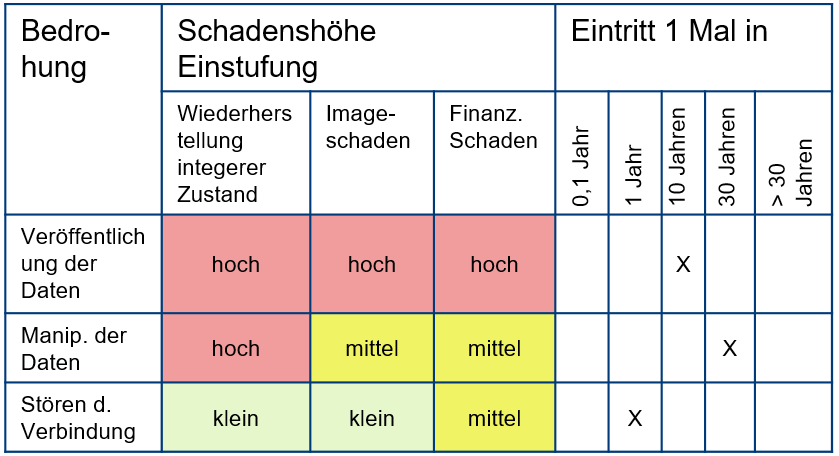
\includegraphics[width= 0.8\textwidth]{Bilder/risikoregister.png}
            \caption{Risiko-Register des Szenarios}
            \label{fig:riskreg}
      \end{center}
\end{figure}


Der gravierendste Fall für das Unternehmen wäre die Veröffentlichung der gesammelten Daten oder die Androhung dessen. Der in Kapitel \ref{Risikoidentifizierung} beschriebene \glqq{}Human Impact\grqq{} wäre
in diesem Fall am höchsten. Da ein Verkehrsbetrieb stark von dem Vertrauen der Fahrgäste abhängig ist, kann der entstehende Imageschaden als hoch eingeordnet werden. Der Aufwand, einen
integeren Zustand wiederherzustellen, ist ebenfalls als hoch anzusehen da gegebenenfalls Teile der Systemarchitektur geändert werden müssen. So entsteht ein hoher finanzieller Schaden, der durch das Schließen
von Sicherheitslücken, Ändern der Systemarchitektur und eventuellen Kosten zur Kompensation des Human Impact entsteht. Da das Beschaffen mit hohem Aufwand verbunden ist aber leicht zur Erpressung genutzt werden kann,
ist die Einschätzung eines Vorkommens von einem Vorfall in 10 Jahren realistisch.


Der nächste Fall ist die Manipulation der Daten, in welcher beispielsweise falsche Aufnahmen gesendet werden. Einen integren Zustand wiederherzustellen ist hier sehr aufwändig, da eine Manipulation der Daten
nicht immer direkt erkennbar ist. Der Imageschaden ist weniger hoch als bei einer möglichen Veröffentlichung, aber dennoch zu berücksichtigen falls die Manipulation publik gemacht wird. So entsteht ein mittlerer
finanzieller Schaden, hauptsächlich bedingt durch die Wiederherstellung des integren Zustands. Durch den hohen Aufwand zur Manipulation der Daten ist diese Bedrohung als verglichen selten einzuordnen.


Die dritte mögliche Option ist das simple Stören der Verbindung. Dies kann durch eine \glqq{}Physical Attack\grqq{} entstehen, beispielweise dem Durchschneiden einer Netzwerkleitung. Die Wiederherstellung des
integeren Zustands ist durch eine Reparatur zu gewährleisten, der Imageschaden ist durch die geringe Signifikanz auch begrenzt und nur der finanzielle Schaden kann leicht ansteigen, durch beschädigtes Material
oder entstehende Wartungskosten. Im Gegensatz zu den vorangehenden Bedrohungen tritt diese allerdings relativ häufig auf, da das Stören einer Verbindung mit wenig \glqq{}Adversary's Resources\grqq{} möglich ist.

\subsection{Maßnahmen}
Da in diesem Szenario die nicht-technischen Systeme der Fahrgastüberwachung, wie Kontrolleure in der Zentrale, weniger stark eine Rolle spielen, kann sich auf die technische Sicherung der Netzwerkverbindung konzentriert werden.
Um Maßnahmen abzuleiten, können die beeinträchtigten Schutzziele des Systems betrachtet werden. Das Stören der Verbindung ist eine Verletzung der Verfügbarkeit (Schutzziel Nr. 2). Um hier die Ausfallsicherheit
zu erhöhen, kann eine Redundanz geschaffen werden. Wenn zwei voneinander getrennte Kommunikationskanäle existieren, wird es schwerer sein
die Verbindung zu stören. Das Schutzziel der Verfügbarkeit wird somit bestärkt.

Um das Schutzziel der Integrität zu bestärken, muss die Architektur des Systems verändert werden. Eine Methode hierbei ist die Verwendung eines \glqq{}Secure Hash Algorithm\grqq{}, einem parametrisierten Hashverfahren.
Der Hash wird vor dem Versenden aus den Eingabedaten und dem Shared key, einem Passwort welches nur der Sender und Empfänger kennen, berechnet. So kann der Empfänger anhand des Hash-Wertes überprüfen,
ob die Nachricht manipuliert wurde, da in diesem Falle der Hash-Wert abweicht. Die Integrität der Daten ist somit optimiert und die Manipulation der Daten kann so erkannt werden.

Um das Schutzziel der Vertraulichkeit zu gewährleisten, muss die Integrität der Daten gegeben sein. Essentiell für das Sicherstellen der Vertraulichkeit ist zudem eine Verschlüsselung. Da in einem Verkehrsbetrieb alle Akteure
bekannt sind (Abschnitt \ref{abschnitt:technisch}: Eine Zentrale und mehrere Netzwerk-Switches in den Fahrzeugen/ Haltestellen), kann eine \glqq{}Public Key Infrastructure\grqq{} verwendet werden. In dieser gibt
eine zentrale Stelle einen öffentlichen Schlüssel heraus, mit welchem die vielen kleinen Akteure ihre Daten verschlüsseln und an die Zentrale senden. Dort werden die Inhalte wieder mit einem private key entschlüsselt.
Dieser Private Key ist im Gegensatz zum Public Key geheim und nicht außerhalb der Zentrale bekannt. Die Authentizität der Keys kann innerhalb des Verkehrsbetriebes sichergestellt werden.